\documentclass[10pt,professionalfonts,serif,usenames,dvipsnames,svgnames,table]{beamer}

\usepackage{hyperref}
\hypersetup{
	pdfpagelabels=false
}

\usetheme{Warsaw}

\definecolor{darkgreen}{rgb}{0, 0.5, 0.0}
\newcommand{\docutilsrolegreen}[1]{\color{darkgreen}#1\normalcolor}
\newcommand{\docutilsrolered}[1]{\color{red}#1\normalcolor}

\newcommand{\green}[1]{\color{darkgreen}#1\normalcolor}
\newcommand{\red}[1]{\color{red}#1\normalcolor}

\usepackage{lmodern}
%\usepackage{garamond}
\usepackage[garamond]{mathdesign}
%\usepackage[urw-garamond]{mathdesign}

%\usepackage{amsmath}
%\usepackage{amssymb}
%\usepackage{amsthm}
%\usepackage{amsfonts}
\usepackage{graphicx}
\usepackage{verbatim}
\usepackage{fancyvrb}
\usepackage{verbments}
\usepackage{colortbl}
\usepackage{slashed}
\usepackage{tabularx}
%\usepackage[normalem]{ulem}
\usepackage{tikz}

\usepackage[loop, autoplay, buttonsize=1em, buttonbg=0, buttonfg=1]{animate}
\usepackage{movie15}

\providecommand\thispdfpagelabel[1]{}

\usetikzlibrary{shapes,arrows,trees}
\hypersetup{
colorlinks=true,
urlcolor=blue,
linkcolor=blue
}

%\usefonttheme[onlymath]{serif}
%\usecolortheme{orchid}
%\useinnertheme{rounded}

%\setbeamertemplate{headline}[default]
\setbeamercolor{author in head/foot}{fg=black,bg=white}
\setbeamercolor{title in head/foot}{fg=black,bg=white}
\setbeamercolor{date in head/foot}{fg=black,bg=white}

%\addtoheadtemplate{\pgfuseshading{beamer@headfade}\vskip-1.25cm}{}
%\usebackgroundtemplate{\includegraphics[width=\paperwidth,height=\paperheight]{images/bg.eps}}

%\setbeamercolor{frametitle}{bg=Blue,fg=white}
%\setbeamercolor{title}{bg=Blue,fg=white}

%\setbeamersize{text margin left=.2cm} 
%\setbeamersize{text margin right=.5cm}

\setbeamertemplate{itemize itemsep}[0.3in]
\setbeamertemplate{itemize parsep}[0.3in]
\setbeamertemplate{enumerate itemsep}[0.3in]
\setbeamertemplate{enumerate parsep}[0.3in]

\setbeamertemplate{navigation symbols}{}
\setbeamersize{text margin left=.2cm,text margin right=.2cm}
\setbeamercovered{transparent}

\newcommand{\maxFrameImage}[1]
{
	{
	\setbeamercolor{background canvas}{bg=black,fg=white}
	\usebeamercolor[fg]{background canvas}
	\begin{frame}[plain]
	\begin{changemargin}{-1cm}{-1cm}
	\begin{center}
	\includegraphics[width=1.01\paperwidth,height=1.01\paperheight,keepaspectratio]{#1}
	\end{center}
	\end{changemargin}
	\end{frame}
	}
}

\newenvironment{changemargin}[2]{
	\begin{list}{}
	{
	\setlength{\topsep}{-3pt}
	\setlength{\leftmargin}{#1}
	\setlength{\rightmargin}{#2}
	\setlength{\listparindent}{\parindent}
	\setlength{\itemindent}{\parindent}
	\setlength{\parsep}{\parskip}
	}
	\item[]
}{\end{list}}

\newenvironment<>{varblock}[2][\textwidth]
{
	\setlength{\textwidth}{#1}
	\begin{actionenv}#3
	\def\insertblocktitle{#2}
	\par
	\usebeamertemplate{block begin}
	}
	{\pa
	\usebeamertemplate{block end}
	\end{actionenv}
}

\defbeamertemplate*{footline}{my theme}
{
  \leavevmode%
  \hbox{%
  \begin{beamercolorbox}[wd=.333333\paperwidth,ht=3.25ex,dp=1.25ex,left]{author in head/foot}%
    \usebeamerfont{author in head/foot}\hspace*{3.25ex}\insertshortauthor~~(\insertshortinstitute)
  \end{beamercolorbox}%
  \begin{beamercolorbox}[wd=.333333\paperwidth,ht=3.25ex,dp=1.25ex,center]{date in head/foot}%
    \usebeamerfont{date in head/foot}%\insertshortdate{}\hspace*{2em}
    {\large\insertframenumber{}}/\inserttotalframenumber{}
  \end{beamercolorbox}}%
  \begin{beamercolorbox}[wd=.333333\paperwidth,ht=3.25ex,dp=1.25ex,right]{title in head/foot}%
    \usebeamerfont{title in head/foot}\insertshorttitle\hspace*{3.25ex}
  \end{beamercolorbox}%
  \vskip0pt%
}


../common/phys_defs.tex

\title{rootpy: Pythonic ROOT}
%\subtitle{I have no subtitle}
\author[Noel Dawe]{Noel Dawe}
\date[\today]{\today}
\institute[rootpy]{for the rootpy dev team}
\titlegraphic{\includegraphics[height=3cm]{../common/images/rootpy_logo.png}}

\begin{document}

\frame{\titlepage
    \begin{center}
    {\bf ROOT Users Workshop, Saas-Fee}
    \end{center}
}

\frame{
    \frametitle{What's the problem?}

    \begin{center}
    {\bf Why would we even consider developing a layer on top of PyROOT?}
    \end{center}

    \begin{itemize}
        \itemsep=.3cm
        \item PyROOT is mainly bindings (although with some pythonization).
        \item Python's dynamic nature provides {\bf many possibilities not
            currently realized by PyROOT}. One might argue a majority of these
            high-level pythonizations are {\bf beyond the scope of what PyROOT should
            offer.}
        \item Certain tasks require awkward code and are error-prone.
            Similar workarounds are implemented by many in multiple places.\\
            {\bf Why not solve these issues once and for all?}
        \item There is a lack of integration of ROOT with the vast and growing
            ecosystem of scientific Python packages.\\ {\bf Why not enable users to
            benefit from both the power of ROOT and what is offered by the
            scientific Python community?}
        \end{itemize}
}

\frame{
    \frametitle{Scientific Python Applications}
    \begin{itemize}
        \item Interactive computing: \href{http://ipython.org/}{IPython}
        \item Powerful and fast array manipulation:
            \href{http://numpy.scipy.org/}{NumPy}
        \item Efficiently and easily handle large amounts of data:
            \href{http://www.pytables.org/moin}{PyTables}
        \item General scientific library: \href{http://www.scipy.org/}{scipy}
        \item Data analysis and modeling: \href{http://pandas.pydata.org/}{pandas}
        \item Statistical models and tests: \href{http://statsmodels.sourceforge.net/}{statsmodels}
        \item Fitting: \href{http://cxc.harvard.edu/sherpa4.4/index.html}{sherpa}
        \item Astronomy: \href{http://www.astropy.org/}{astropy}
        \item Image processing: \href{http://scikit-image.org/}{scikit-image}
        \item Machine learning:
            \href{http://scikit-learn.org/stable/}{scikit-learn}
        \item Feature-rich publication-quality plotting:
            \href{http://matplotlib.org/}{matplotlib}
        \item See a list of other kits here:
            \href{http://scikits.appspot.com/scikits}{scikits.appspot.com/scikits}
    \end{itemize}
}

\frame{
    \frametitle{Introducing rootpy}

    \begin{itemize}
        \item rootpy aims to provide a \textbf{\emph{ more pythonic layer}} on
            top of the PyROOT bindings and to take advantage of advanced
            features of the Python language.
        \item {\bf rootpy does not intend to recreate ROOT} or to {\em severely}
            alter the default behaviour of ROOT.
        \item {\bf rootpy is not an analysis framework}, but rather a library that
            one's analysis framework might use.
        \item rootpy provides an {\bf interface with the scientific Python
            packages}:
        \end{itemize}
        \begin{center}
            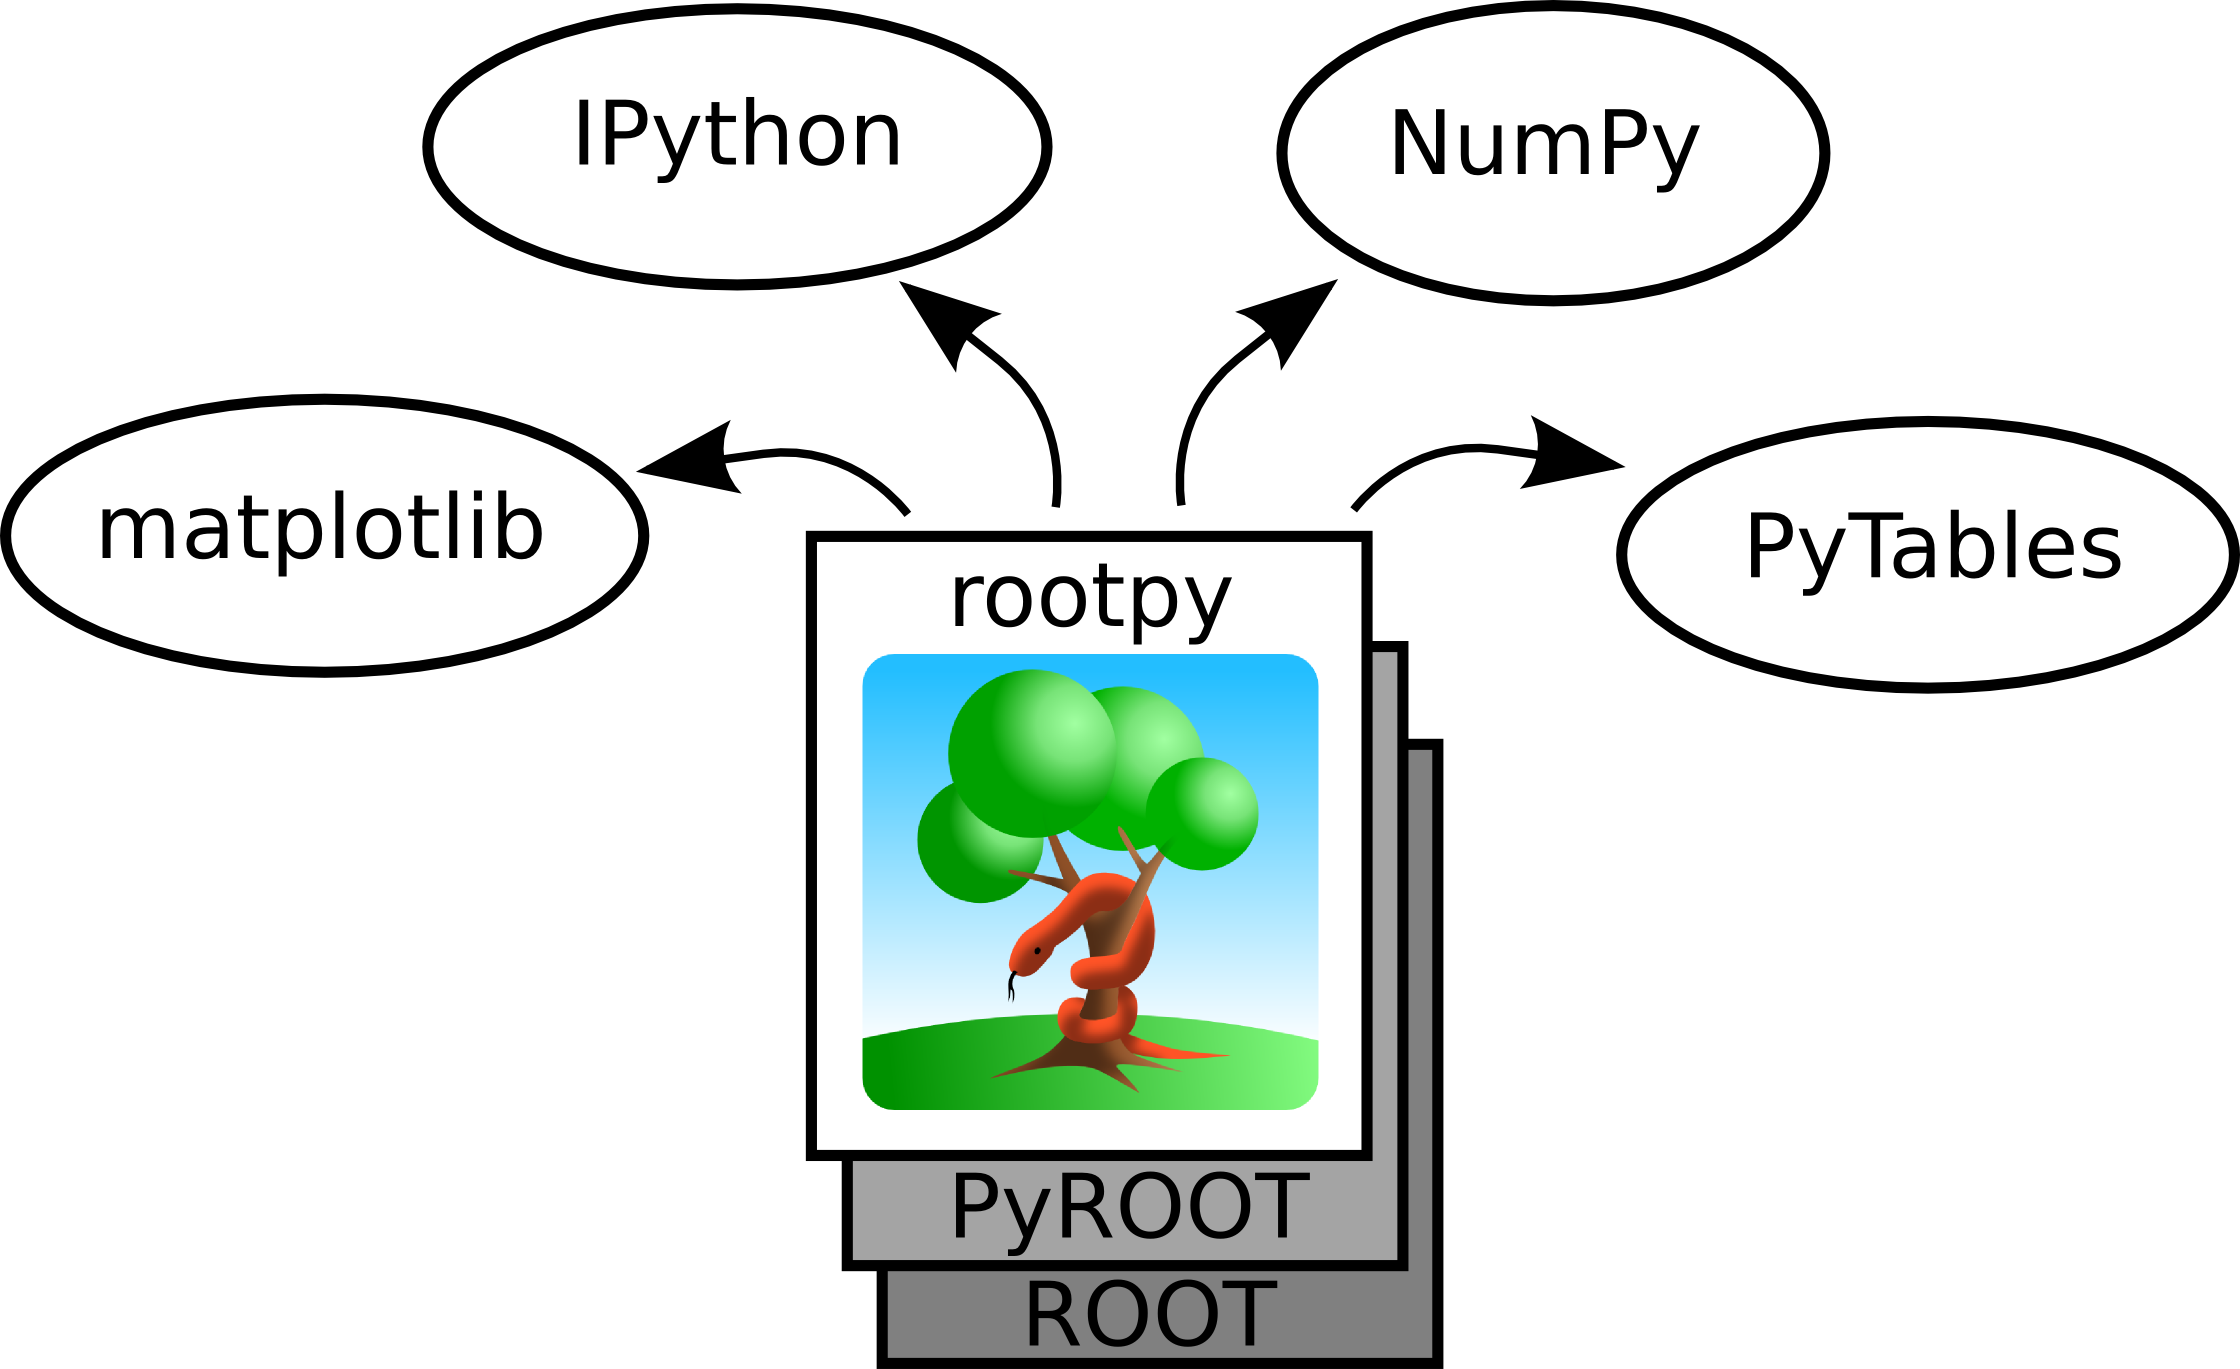
\includegraphics[width=.5\textwidth]{figs/rootpy-map.png}
        \end{center}
}

\frame{
    \frametitle{rootpy: key concepts and design philosophy}

    \begin{itemize}
        \item Pythonized classes in rootpy are subclasses of the corresponding
            ROOT classes with the same (or similar) name without the ``T''.\\
            (for example: TFile $\rightarrow$ File, TCanvas $\rightarrow$ Canvas, \\
            TH[1|2|3][C|S|I|F|D] $\rightarrow$ Hist, Hist2D, Hist3D).
        \item ROOT methods may be overridden or new methods created to add
            functionality (i.e. operators) and objects may be decorated with
            additional properties.
        \item Object names and titles are optional. Unspecified names default to
            UUIDs.
        \item ROOT messages should be routed through Python's logging system
            with error messages raised as Python exceptions.
        \item Python has a garbage collector but C++ does not: this can lead to
            strange issues. rootpy addresses these problems.
        \item Anywhere Python is typically slow we intend to instead use
            compiled C extension modules. Through the root\_numpy
            package, rootpy provides very fast conversion of ROOT Trees into
            NumPy arrays as well as efficiently filling ROOT histograms with
            NumPy arrays.
        \end{itemize}
}

\frame{
    \frametitle{What does rootpy offer?}

    \begin{center}
    \rowcolors[]{1}{blue!20}{blue!10}
    \begin{tabular}{l p{8cm}}
        {\bf rootpy.plotting} & histogram, graphs, canvas, pad, legend, and
            style subclasses with additional pythonizations,
            functions for plotting ROOT histograms with matplotlib. \\
        {\bf rootpy.tree} & trees, chains, tree objects, tree models, cuts. \\
        {\bf rootpy.io} & file and directory subclasses, utilities. \\
        {\bf rootpy.logger} & routing ROOT messages through Python's
            logging module. Turn ROOT error messages into Python exceptions. \\
        {\bf rootpy.memory} & utilities for monitoring TObject deletions
            and for keeping objects alive when explicit references on the Python
            side go out of scope. \\
        {\bf rootpy.interactive} & a wait function for preventing Python
            from exiting until all canvases have been closed. \\
        {\bf rootpy.root2hdf5} & conversion of ROOT files to HDF5. \\
        {\bf rootpy.context} & utilities for managing ROOT's global state. \\
        \multicolumn{2}{c}{\ldots and more \ldots} \\
        \end{tabular}
    \end{center}
}

\begin{frame}[fragile]
    \frametitle{rootpy example: opening a TFile}
    \begin{footnotesize}
\begin{minted}{python}
from rootpy.testdata import get_file

# use the test file shipped with rootpy
with get_file() as f:
    # access objects by name as properties of the current dir
    myhist = f.dimensions.hist2d
    # recursively walk through the file
    for path, dirs, objects in f.walk():
        # do something
        print path, dirs, objects
\end{minted}
\end{footnotesize}

\end{frame}

\begin{frame}[fragile]
    \frametitle{rootpy example: creating histograms}
    \begin{footnotesize}
\begin{pyglist}[language=python,texcl=true,abovecaptionskip=0,style=vs,bgcolor=Moccasin]
from ROOT import TH3D
from array import array

# variable width bins
hist3d = TH3D('3d', '3d', 3, array('d', [0, 3, 10, 100]),
                          5, array('d', [2.3, 4.2, 5.8, 10, 20, 25.5]),
                          2, array('d', [-100, 0, 20]))
# ROOT is missing some constructors... (the following will not work)
hist3d = TH3D('3d', '3d', 3, 0, 5,
                          5, array('d', [2.3, 4.2, 5.8, 10, 20, 25.5]),
                          2, array('d', [-100, 0, 20]))
\end{pyglist}
\end{footnotesize}

    \begin{footnotesize}
\begin{pyglist}[language=python,texcl=true,style=vs,bgcolor=Moccasin]
from rootpy.plotting import Hist3D

# variable width bins
hist3d = Hist3D([0, 3, 10, 100], [2.3, 4.2, 5.8, 10, 20, 25.5], [-100, 0, 20])
# easy to mix variable and fixed width bins with rootpy
hist3d = Hist3D(3, 0, 5, [2.3, 4.2, 5.8, 10, 20, 25.5], [-100, 0, 20])
\end{pyglist}
\end{footnotesize}

\end{frame}

\begin{frame}[fragile]
    \frametitle{rootpy example: filling a TTree}
    \begin{footnotesize}
\begin{pyglist}[language=python,texcl=true,abovecaptionskip=0,style=vs,bgcolor=Moccasin]
from array import array
from random import gauss

output_file = TFile.Open('output.root', 'recreate')
some_float = array('f', [0.])
some_int = array('i', [0])
tree = TTree('mytree', '')
tree.Branch('some_float', some_float, 'some_float/F')
tree.Branch('some_int', some_int, 'some_int/I')

for i in xrange(100):
    some_float[0] = gauss(0, 1)
    some_int[0] = i
    tree.Fill()

tree.Write()
output_file.Close()
\end{pyglist}
\end{footnotesize}

\end{frame}

\frame{
    \frametitle{The future of rootpy}

    \begin{itemize}
        \item Larger documentation coverage. This is important!
        \item More code examples.
        \item Python 3 support.
        \item Better integration with the IPython prompt: full tab completion
            and helpful builtin commands like pylab.
        \item Automatic wrapping of ROOT methods by parsing method signatures:
            \begin{itemize}
                \item If a method expects a TColor, rootpy can accept any matplotlib/ROOT color
                      and convert it into a TColor before passing to the ROOT method.
                \item Reduce the amount of code in rootpy.
                \end{itemize}
       \item TMVA:
           \begin{itemize}
                \item Ability to feed TMVA classifiers NumPy arrays.
                \end{itemize}
       \item RooFit and RooStats:
           \begin{itemize}
                \item Wrap RooArgSet as set() and RooArgList as list()?
                \item Create RooDataSets from NumPy arrays.
                \end{itemize}
   \end{itemize}
}

\begin{frame}[fragile]
    \frametitle{How can you contribute?}

    \begin{center}
    
\includegraphics[width=5cm]{figs/we-want-you.jpg}
    \end{center}

    \begin{itemize}
        \item Development is community-driven.
        \item We use Git! See the rootpy collaboration on GitHub:
            \href{https://github.com/rootpy}{github.com/rootpy}
        \item Just fork rootpy into your own GitHub account and:
            \begin{pyglist}[language=bash,texcl=true,style=vim]
git clone git@github.com:<username>/rootpy.git
            \end{pyglist}
              Then submit a pull request with your contribution.
        \item Contributions are reviewed by peers before merging into the main branch.
        \item All new code is automatically tested against our test suite using
            \href{https://travis-ci.org/}{Travis CI}.
    \end{itemize}
\end{frame}

\end{document}
